\documentclass[parskip=full,11pt,twoside]{scrartcl}
\usepackage[utf8]{inputenc}

\title{VIPER: Viper Interactive Prolog Education Runtime}
\author{Paul Brinkmeier, Luke Brocke, Christian Oder, Aaron Maier, Jannik Koch}

% section numbers in margins:
\renewcommand\sectionlinesformat[4]{\makebox[0pt][r]{#3}#4}

% header & footer
\usepackage{scrlayer-scrpage}
\lofoot{\today}
\refoot{\today}
\pagestyle{scrheadings}

\usepackage{amsmath} % for $\text{}$

\usepackage[sfdefault,light]{roboto}
\usepackage[T1]{fontenc}
\usepackage[german]{babel}
\usepackage[yyyymmdd]{datetime} % must be after babel
\renewcommand{\dateseparator}{-} % ISO8601 date format
\usepackage{hyperref}
\usepackage[nameinlink]{cleveref}
\crefname{figure}{Abb}{Abb}
\usepackage[section]{placeins}
\usepackage{xcolor}
\usepackage{graphicx}
\usepackage{listings}
\usepackage{courier}
\hypersetup{
	pdftitle={Pflichtenheft},
	bookmarks=true,
}
\usepackage{csquotes}

\newcommand\urlpart[2]{$\underbrace{\text{\texttt{#1}}}_{\text{#2}}$}

\usepackage{pflichtenheft}

\lstset{language=Prolog}
\lstset{basicstyle=\ttfamily,breaklines=true}

\begin{document}
\maketitle

\section{Einleitung}

Prolog ist eine logische Programmiersprache die ein deklaratives Programmieren ermöglicht.

Das Grundprinzip von Prolog besteht aus einer Wissensdatenbank, deren Einträge sich Fakten und Regeln nennen.

\begin{lstlisting}
father(homer, bart).
father(abe, homer).
\end{lstlisting}

So gilt, dass Homer der Vater von Bart ist und Abe der Vater von Homer.

Für eine Abfrage erhalten wir also folgende Ergebnisse:
\begin{lstlisting}
?- father(homer, bart).
yes .
?- father(bart, abe).
no .
\end{lstlisting}

Nun ist es möglich, Relationen basierend auf Fakten einzuführen. Setzen wir also Großvater für alle Väter von Vätern indem wir Variablen benutzen.
\begin{lstlisting}
grandfather(X, Y) :- father(X, Z), father(Z, Y).
\end{lstlisting}

Selbiges ist möglich für Abfragen.
\begin{lstlisting}
?- father(X, bart).
X = homer .
?- father(X, Y).
X = homer, Y = bart ;
X = abe, Y = homer .
?- grandfather(X, Y).
X = abe, Y = bart .
\end{lstlisting}

Die Antworten sind alle möglichen Kombinationen aus den Variablen die den Fakten und Relationen entsprechen.

Prolog ist hierbei anders als \enquote{andere} Programmiersprachen, da es sich um eine deklarative Programmiersprache handelt. Die Relationen basieren auf zuvor definierten Fakten.

VIPER, die VIPER Interactive Prolog Education Runtime, ist ein Programm zur Bearbeitung und dem Testen von einfachen Prolog-Programmen. Über die visuelle Schnittstelle ist es dem Nutzer möglich, Prolog zu schreiben, Abfragen zu stellen und diese visualisieren zu lassen.

Dank des automatisch generierten Graphen ist es dem Nutzer hierbei möglich, die Interpretation des Programmes schrittweise anzuzeigen und nachzuvollziehen.

Damit soll dem Nutzer die Funktionsweise von Prolog-Programmen durch die graphische Visualisierung näher gebracht werden und zum verbesserten Verständnis von Prolog beitragen.

\pagebreak
\section{Kriterien}
% Diese Section sollte kurz und knapp "für Manager" sein
% und auf eine Seite passen.

\subsection{Muss}

\criterium{Öffnen}{crt:open}

Das Programm soll bereits vorhandene Prolog-Programme öffnen können, damit auf diesen Abfragen durchgeführt und diese visualisiert werden können.

\criterium{Speichern}{crt:save}

Das Programm soll Änderungen am momentan geladenen Prolog-Programm speichern können. Dabei soll geprüft werden ob das Prolog-Programm seit dem Laden schon anderweitig verändert wurde und sollte dies der Fall sein wird eine Warnung ausgegeben.

\criterium{Interpretation eines Prolog-Programms mit begrenztem Umfang}{crt:interpretation}

% Verweis auf Glossareintrag
Das Programm kann eine Teilmenge der Prologsprache interpretieren:

Es gibt IDs, Variablen und Zahlen die wie folgt notiert werden:

id := [a-z][a-zA-Z0-9]*\newline
var := [A-Z][a-zA-Z0-9]*\newline
num := [0-9]*

Es gibt Terme welche sich aus obigem zusammensetzen:

Term := Funktor | var | num\newline
Funktor := id | id( Term\{, Term\}* )

Und zusätzlich gibt es Regeln und Ziele welche sich wie folgt zusammensetzen:

Regel := Funktor . | Funktor :- Ziel \{, Ziel\}* .\newline
Ziel := Funktor | Term = Term

Anmerkung: Eine Regel die nur aus einem Funktor ohne Ziel besteht wird Fakt genannt.

\criterium{Einzelschritt-Interpreter}{crt:interpreter}

% Verweis auf GUI und mögliche Anpassung des Buttonnamens
Das Programm bearbeitet Anfragen schrittweise. Nach jedem durchgeführten Teilschritt einer Abfrage wartet das Programm auf Interaktion vom Nutzer (drücken des "Verarbeiten" Buttons) bis es den nächsten Teilschritt bearbeitet.

\criterium{Visualisierung}{crt:visualization}

% Verweise auf GUI
Das Programm kann Abfragen zu einem Prolog-Programm mit Hilfe eines Graphen visualisieren. Dieser hat eine Baumstruktur und beinhaltet für jeden Abarbeitungsschritt einen eigenen Knoten.

\criterium{Listen}{crt:lists}

Das Programm unterstützt die Darstellung von Listen. Die leere Liste wird durch \enquote{[]} dargestellt, eine Liste mit Inhalt wird durch \enquote{[1,2,3]} dargestellt und intern als Listenkopf und \enquote{Restliste} behandelt, das heißt:\newline
Liste: \enquote{[1,2,3]}\newline
In Prolog: \enquote{[1|teilliste1]}, teilliste1= \enquote{[2|teilliste2]}, teilliste2=[3]

\subsection{Kann}

\criteriumOptional{Zurückschreiten}{crt:stepback}

% Verweis auf GUI
Das Programm soll es dem Nutzer ermöglichen die letzten 5 Schritte schrittweise zurückzugehen um z.B. Zustandsunterschiede im Graphen besser erklären zu können.

\criteriumOptional{Ausführung bis zur nächsten Ausgabe}{crt:continueto}

% Verweis auf GUI
Das Programm soll durch einen extra Knopf bis zur nächsten Ausgabe ausgeführt werden können.

\criteriumOptional{X Ausführungen}{crt:multistep}

% Verweis auf GUI
Das Programm soll durch einen extra Knopf X Schritte auf einmal ausführen.

\criterium{Abbrechen}{crt:cancel}

% Verweis auf GUI
Das Abarbeiten eines Teilschritts soll durch einen Knopfdruck abgebrochen werden können, falls dieser z.B. viele Rekursionen beinhaltet und deswegen eine lange Bearbeitungszeit hat.

\criteriumOptional{Cut}{crt:cut}

Das Programm soll die "Cut"-Funktionalität unterstützen, mit der der Nutzer dem Programm, durch das Hinzufügen eines "!" am Ende einer oder mehrerer Regeln bzw. Ziele, verbieten kann bei der Abarbeitung auf diese Regel(-n)/Ziele zurück zu springen.

\criteriumOptional{Arithmetik}{crt:maths}

Das Programm soll grundlegende Arithmetik unterstützen. Da Terme in Prolog nur für sich selber stehen können Abfragen wie "4 = 1 + 3" nicht bearbeitet werden. Daher wird das Programm um einen Term \enquote{is} erweitert welcher solche arithmetischen Abfragen ermöglicht.

\criteriumOptional{Standardbibliothek}{crt:standardlib}

Das Programm soll eine kleine Standardbibliothek mit nützlichen, vordefinierten, Regeln unterstützen die standardmäßig beim Starten des Programms mit eingebunden wird.

\criteriumOptional{Standardbibliothek deaktivieren}{crt:disablelib}

Das Programm soll es dem Nutzer ermöglichen die eingebundene Standardbibliothek deaktivieren zu können.

\criteriumOptional{Export von Visualisierungsbäumen als LaTeX-Code}{crt:latex}

Das Programm kann einen Visualisierungsbaum als LaTeX-Code exportieren, damit dieser vereinfacht in Dokumente eingebunden werden kann.

\criteriumOptional{Export von Visualisierungsbäumen als Bilddatei}{crt:export}

Das Programm kann einen Visualisierungsbaum als Bilddatei im SVG/PNG-Format exportieren.

\criteriumOptional{Syntaxhighlighting}{crt:syntaxhighlighting}

Das Programm soll das farbliche hervorheben bestimmter Regeln und ihres/ihrer korrepsondieren Knoten in der Visualisierung unterstützen. Der Code wird dabei farblich passend hervorgehoben. Identifier und Variablen werden dabei unterschiedlich zu Zahlen eingefärbt. Ebenfalls unterscheiden sich die Farben von umschließenden Klammern. Die Operatoren \texttt{=}, \texttt{:-}, \texttt{is} und \texttt{!} sind farblich von allem anderen unterscheidbar.

\criteriumOptional{"Pretty-Printing" von Listen}{crt:prettyprinting}

Das Programm soll Listen bei der Ausgabe einheitlich auf \enquote{[x,y,z]} formatieren.

\subsection{Abgrenzung}

\criteriumNot{Voller Sprachsupport}{crt:fullsupport}

Die Software hat kein Verständnis für Prolog-Sprachfeatures außerhalb der vorgestellten Prolog-Teilmenge.

\criteriumNot{Andere Programmiersprachen}{crt:otherlanguages}

Die Entwicklungsumgebung beschränkt sich auf die Prolog-Sprache und bietet keine offiziell Unterstützung für Prolog-Dialekte oder andere Programmiersprachen jeglicher Art.

\criteriumNot{Nutzung in einer Kommandozeile}{crt:cli}

Das Produkt beschränkt sich auf eine graphische Darstellung über GUI-Elemente. Eine Interaktion über die Konsole ist nicht unterstützt.

\criteriumNot{Professionelle Anwendung}{crt:professionaluse}

Die Software ist nicht für professionelle Anwendungszwecke ausgelegt.

\pagebreak
%%%%%%%%%%%%%%
\section{Produkteinsatz}

Das Produkt soll als graphisches Prolog-Lerntool betrieben werden.

Die Zielgruppe des Lerntools sind Lehrende, Studierende und Enthusiasten.

Das Produkt soll sich auf eine Teilmenge der Prolog-Sprache beschränken, diese jedoch voll unterstützen.

Das Produkt soll für die Teilmenge der Sprache eine Lernhilfe sein und das Verständnis für die Funktionsweise von Prolog, mit Hilfe von schrittweiser Visualisierung, stärken.

Das Produkt ermöglicht es mit Hilfe eines eingebauten Editors Prolog-Programm zu bearbeiten und zu erweitern.

\section{Produktumgebung}

Das Programm soll als graphische Applikation auf einem Desktop-System betrieben werden.

Es stehen mindestens 2 AMD64/x86 Kerne mit insgesamt 2GB shared RAM zur Verfügung.

Unterstützte Betriebssysteme sind Windows ab Version 7 und aufwärts, Mac OSX 10.9 aufwärts sowie Ubuntu Linux 16.04.

Eine Maus sowie eine Tastatur sind als Eingabegeräte angeschlossen und funktionsfähig.

Eine Installation des Java Runtime Environments Version 8 aufwärts ist auf dem System vorhanden.

\newpage

%%%%%%%%%%%
\section{Produktdaten}

\textbf{Zuletzt geöffnete Dateien} \\
Die Pfade der fünf zuletzt geöffneten Dateien werden für einen Eintrag im Kontextmenü gespeichert.

Außer den oben gennanten werden keinerlei Daten gespeichert.
%%%%%%%%%%%
\section{Funktionale Anforderungen}

\functionality{Erstellen eines neuen Editor-Puffers}{fnc:new}
\fulfills{crt:new}

Die Software stellt einen Editor bereit, in dem ein leerer Puffer angelegt werden kann. Sollte der Puffer zuvor bereits ungesicherten Inhalt besitzen, so wird der Nutzer aufgefordert, diesen zu speichern. Der alte Puffer wird daraufhin verworfen und ein leerer Puffer geladen.

\functionality{Öffnen einer Prolog Quellcode-Datei}{fnc:open}
\fulfills{crt:open}

Die Software ist in der Lage, Prolog-Quelltext-Dateien zu öffnen. Der Datei-Inhalt wird dabei in den Puffer des Editors geladen und angezeigt. Analog zur Erstellung eines neuen Puffers wird, falls nötig, zur Speicherung ungesicherter Inhalte aufgefordert und der alte Puffer daraufhin verworfen.

\functionality{Öffnen einer zuletzt verwendeten Prolog Quellcode-Datei}{fnc:recentfiles}
\fulfills{crt:recentfiles}

Die Software bietet ein Kontextmenü für den Schnellzugriff auf bis zu fünf der zuletzt verwendeten Dateien an. Diese können über dieses Menü einzeln analog zu F2 in das Editor-Fenster geladen werden. Sollten kürzlich verwendete Dateien verschoben oder gelöscht werden, so werden diese in besagtem Kontext-Menü nicht angezeigt.

\functionality{Verändern des Editor-Puffers}{fnc:editor}
\fulfills{crt:save}

Der Puffer-Inhalt des Editors kann bearbeitet werden. Dies verändert ausschließlich den Editor-Puffer.

\functionality{Speichern des Editor-Inhalts}{fnc:save}
\fulfills{crt:save}

Die Software kann den Inhalt des Editor-Puffers auf die Festplatte schreiben. Wurde der Editor-Puffer bisher noch nicht gespeichert, so kann dieser über einen Auswahldialog in eine neue Datei gespeichert werden. Entspricht der Editor-Inhalt einer bereits existierenden, geöffneten Datei, so wird der Inhalt dieser Datei überschrieben. Wurde die Datei seit dem Öffnen anderweitig geändert (bspw. durch einen anderen Text-Editor), verändert dies den Editor-Puffer nicht. Für eine Aktualisierung des Puffer-Inhalts muss die Datei erneut geöffnet werden.

\functionality{Parsen einer im Editor geöffneten Prolog Datei}{fnc:parser}
\fulfills{crt:parser}

Der Inhalt einer geöffneten Datei kann durch einen Parser verarbeitet werden. Dies geschieht über eine Parse-Schaltfläche im Editor. Wird der Parser über diese Schaltfläche gestartet, werden die Fenster der Konsole und der Visualisierung geleert. Ungesicherte Editor-Puffer müssen vor der Verarbeitung mit dem Parser gespeichert werden.

\functionality{Fehlerausgabe beim Parsen einer inkorrekten Prolog Datei}{fnc:errorcheck}
\fulfills{crt:errorcheck}

Der Parser erkennt Fehler innerhalb einer geöffneten Prolog-Datei bei der Verarbeitung. Fehlermeldungen werden über das verfügbare Konsolen-Fenster ausgegeben.

\functionality{Eingabe von Prolog-Abfragen in die Konsole}{fnc:shell}
\fulfills{crt:shell}

Bei erfolgreicher Verarbeitung einer fehlerfreien Datei durch den Parser erlaubt die angezeigte Konsole die Eingabe von Abfragen. Sollten erneut Änderungen an der geladenen Prolog-Datei stattfinden und gespeichert werden, so wird die Eingabe in die Konsole sowie jegliche Interaktion mit der Visualisierung gesperrt bis der veränderte Quelltext erneut vom Parser verarbeitet wurde.

\functionality{Interpretation von Prolog-Abfragen in der Konsole}{fnc:interpreter}
\fulfills{crt:interpreter}

Abfragen, welche in der Konsole eingegeben wurden, werden nach einer Bestätigung mit der Enter-Taste schrittweise interpretiert. Ausgaben des Interpreters werden in der Konsole angezeigt. Nach dem Betätigen der Schaltfläche wird ausschließlich der erste Interpretationsschritt durchgeführt. Der Nutzer hat die Möglichkeit, diese Interpretation über eine Schritt-Schaltfläche schrittweise fortzuführen. Fehler bei der Interpretation einer Abfrage werden über das Konsolen-Fenster ausgegeben und die weitere Verarbeitung wird abgebrochen.

% TODO: Visualisierung genauer!
\functionality{Visualisieren des aktuellen Interpretationsschritts mittels eines Graphen}{fnc:graph}
\fulfills{crt:graph}

Bei aktiver Interpretation einer Abfrage wird eine Visualisierung für den aktuellen Interpretationsschritt generiert und im Visualisierungs-Fenster angezeigt. Sollte zuvor eine Visualisierung in diesem Fenster angezeigt worden sein, wird diese aus dem Fenster gelöscht.

\functionality{Vergrößern und Verkleinern des visualisierten Graphen durch Schaltflächen oder das Mausrad}{fnc:zoom}
\fulfills{crt:zoom}

Über die Verwendung des Mausrads oder der Plus- und Minus-Schaltflächen lässt sich der angezeigte Ausschnitt des Visualisierungs-Graphen vergrößern oder verkleinern.

\functionality{Navigation des visualisierten Graphen durch Bewegungen mit der Maus}{fnc:move}
\fulfills{crt:zoom}

Durch Drücken und Halten der linken Maustaste lässt sich der angezeigte Ausschnitt des Visualisierungs-Graphen bewegen, wodurch der Graph navigiert werden kann.

\functionality{Zurückschreiten während der Interpretation}{fnc:stepback}
\fulfills{crt:stepback}

Eine Rückschritt-Schaltfläche erlaubt bei Betätigung den letzten Schritt rückgängig zu machen. Im Falle des ersten Schrittes hat das Betätigen dieser Schaltfläche keinen Effekt.

\functionality{Ausführung der Interpretation bis zur nächsten Ausgabe}{fnc:continue}
\fulfills{crt:continue}

Eine Fortsetzen-Schaltfläche erlaubt bei Betätigung, die Ausführung bis zur nächsten Ausgabe fortzuführen.

\functionality{Ausführung einer gegebenen Anzahl Schritte während der Interpretation}{fnc:multistep}
\fulfills{crt:multistep}

% TODO: Gibt es eine Schrittzahl ab der Weiterlaufen keinen Effekt mehr hat? Was passiert ab da?
Eine Mehrfachschritt-Schaltfläche öffnet bei Betätigung einen Eingabe-Dialog zur Spezifikation einer Schrittzahl. Nach der Eingabe einer gültigen, ganzen Zahl größer Null wird die spezifizierte Anzahl an Schritten ausgeführt.

\functionality{Abbrechen einer Interpretation}{fnc:cancel}
\fulfills{crt:cancel}

Im Falle einer Interpretation die mehrere Schritte hintereinander ausführt (Mehrfachschritt oder Fortsetzen bis zur nächsten Ausgabe), kann die laufende Interpretation über eine Abbrechen-Schaltfläche frühzeitig beendet werden.

\functionality{Exportieren der angezeigten Visualisierung in einem beliebigen Schritt als Grafik}{fnc:imageexport}
\fulfills{crt:imageexport}

Der aktuell angezeigte Visualisierungs-Graph lässt sich als Bild im PNG- oder SVG-Format exportieren.

\functionality{Exportieren der angezeigten Visualisierung in einem beliebigen Schritt als LaTex-Dokument}{fnc:latexexport}
\fulfills{crt:latexexport}

Der aktuell angezeigte Visualisierungs-Graph lässt sich als LaTex-Dokument exportieren.

\functionality{Deaktivierung der Standardbibliothek}{fnc:disablelib}
\fulfills{crt:disablelib}

Die automatisch eingebundene Standardbibliothek kann über eine Schaltfläche deaktiviert werden. Von der Standardbibliothek zur Verfügung gestellte Funktore werden nun nicht mehr berücksichtigt.

\functionality{Formatierung des Quellcodes}{fnc:formatter}
\fulfills{crt:formatter}

Eine automatische Formatierung von Prolog-Quellcode ist über eine Schaltfläche möglich. Die Formatierung ist hierbei vorgegeben und kann nicht verändert werden. Die Formatierung sieht folgendes vor: Jede Regel wird in ihre eigene Zeile gelegt. Hat eine Regel mehrere Teilziele, so wird die Regelzeile nach dem \enquote{:-}-Operator umgebrochen und alle Teilziele werden in eigene Zeilen gelegt, welche mit zwei Leerzeichen eingerückt sind. Bereits gesetzte Leerzeilen werden beibehalten. Fehlende Leerzeichen vor und hinter dem \enquote{:-}-Operator sowie nach Kommata in Parameterlisten werden eingefügt.

\functionality{Wechsel zwischen den Sprachen Deutsch und Englisch als die in der grafischen Oberfläche verwendete Sprache}{fnc:translation}
\fulfills{crt:translation}

\functionality{Dynamisches Skalieren des Hauptfensters mit der Maus}{fnc:resizeable}
\fulfills{crt:resizeable}

%%%%%%%%%%%
\section{Nicht-Funktionale Anforderungen}

\nonFunctionality{Die VIPER Software startet auf einem modernen System innerhalb von 30 Sekunden und ist voll einsatzbereit.}{nfc:startup}

\nonFunctionality{Ein importiertes oder geschriebnes Prolog Programm ohne Verwendung von Rekursion und im Umfang von maximal 100 Zeilen Code ist innerhalb von maximal 3 Sekunden interpretiert und innerhalb von weiteren 5 Sekunden visualisiert.}{nfc:timelimit}

\nonFunctionality{Das Design wirkt modern und ansprechend.}{nfc:design}

\nonFunctionality{Die Software lässt sich ohne die manuelle Installation weiterer Software durch das Ausführen einer .jar Datei starten.}{nfc:installation}

\nonFunctionality{Die Software ist ohne Abhängigkeiten kleiner als 50 MiB, mit Abhängigkeiten kleiner als 200 MiB.}{nfc:filesize}

\nonFunctionality{Das Laden einer Prolog Datei mit einer Größe von unter 1 MiB geschieht in unter 5 Sekunden.}{nfc:loadfile}

\nonFunctionality{Fehlerhafte Prolog-Programme sollen nie zu einem Absturz des Programms führen.}{nfc:crashresistance}

\nonFunctionality{Der Prolog Interpreter lässt sich in seiner Funktionalität einfach erweitern, um weitere Sprachfeatures zu unterstützen.}{nfc:extendable}

\pagebreak
\section{Tests}

\test{Öffnen einer Prolog-Textdatei}{tst:open}
\tests{fnc:open}

\teststep{Das Programm wird ausgeführt und ist fokussiert. Es ist kein Programm im Editor geöffnet.}
{Der Nutzer wählt über das Datei-Kontextmenü die Öffnen-Funktion aus.}
{Ein Datei-Auswahldialog öffnet sich.}

\teststep{Der Nutzer hat eine Datei über das Auswahlfenster ausgewählt.}
{Der Nutzer betätigt den Öffnen-Button.}
{Die Datei wird im Editor-Fenster geöffnet.}

%%%%%%%%%%%%%%%%%%%%%%%%%%%%%%%%%%%%%%%%%%%%%%%%%%%%%%%%%%%%%%%%%%%%%%%

\test{Öffnen einer Prolog-Textdatei während im Editor bereits ein Programm eingegeben wurde mit Speichern des geschriebenen Programmes}{tst:openanother}
\tests{fnc:open}

\teststep{Das Programm wird ausgeführt und ist fokussiert. Im Editor wurde ein Programm händisch eingegeben.}
{Der Nutzer wählt über das Datei-Kontextmenü die Öffnen-Funktion aus.}
{Ein Datei-Auswahldialog öffnet sich.}

\teststep{Der Nutzer hat eine Datei über das Auswahlfenster ausgewählt.}
{Der Nutzer betätigt den Öffnen-Button.}
{Ein Dialogfenster fragt den Nutzer, ob das im Editor eingegebene Programm gespeichert oder verworfen werden soll.}

\teststep{Der Nutzer hat die Wahl das im Editor geschriebene Programm zu speichern oder zu verwerfen.}
{Der Nutzer betätigt den Speichern-Knopf.}
{Ein Datei-Speichern-Dialog öffnet sich.}

\teststep{Ein Datei-Speichern-Dialog ist geöffnet.}
{Der Nutzer wählt einen Speicherort und wählt einen Dateinamen. Anschließend betätigt es den Speichern-Knopf.}
{Das im Editor geöffnete Programm wird in die gewählte Datei gespeichert. Die zu öffnende Datei wird in den Editor geladen und überschreibt den bisherigen Inhalt.}

%%%%%%%%%%%%%%%%%%%%%%%%%%%%%%%%%%%%%%%%%%%%%%%%%%%%%%%%%%%%%%%%%%%%%%%

\test{Öffnen einer Prolog-Textdatei während im Editor bereits ein Programm eingegeben wurde mit Verwurf des geschriebenen Programmes.}{tst:openanother2}
\tests{fnc:open}

\teststep{Das Programm wird ausgeführt und ist fokussiert. Im Editor wurde ein Programm händisch eingegeben.}
{Der Nutzer wählt über das Datei-Kontextmenü die Öffnen-Funktion aus.}
{Ein Datei-Auswahldialog öffnet sich.}

\teststep{Der Nutzer hat eine Datei über das Auswahlfenster ausgewählt.}
{Der Nutzer betätigt den Öffnen-Button.}
{Ein Dialogfenster fragt den Nutzer, ob das im Editor eingegebene Programm gespeichert oder verworfen werden soll.}

\teststep{Der Nutzer hat die Wahl das im Editor geschriebene Programm zu speichern oder zu verwerfen.}
{Der Nutzer betätigt den Verwerfen-Knopf.}
{Das im Editor geöffnete Programm wird verworfen. Die zu öffnende Datei wird in den Editor geladen und überschreibt den bisherigen Inhalt.}

%%%%%%%%%%%%%%%%%%%%%%%%%%%%%%%%%%%%%%%%%%%%%%%%%%%%%%%%%%%%%%%%%%%%%%%

\test{Syntaktische Hervorhebung von Prolog-Stichworten}{tst:syntaxhighlighting}
\tests{fnc:syntaxhighlighting}

\teststep{Der Nutzer hat ein leeres Editor-Fenster vor sich.}
{Der Nutzer gibt ein gültiges Prolog Programm im Editor ein.}
{Der Code wird farblich passend hervorgehoben. Identifier und Variablen werden dabei unterschiedlich zu Zahlen eingefärbt. Ebenfalls unterscheiden sich die Farben von umschließenden Klammern. Die Operatoren \texttt{=}, \texttt{:-}, \texttt{is} und \texttt{!} sind farblich von allem anderen unterscheidbar.}

%%%%%%%%%%%%%%%%%%%%%%%%%%%%%%%%%%%%%%%%%%%%%%%%%%%%%%%%%%%%%%%%%%%%%%%

\test{Speichern eines im Editor geschrieben Programmes}{tst:save}
\tests{fnc:save}

\teststep{Das Programm wird ausgeführt und ist fokussiert. Ein Programm ist im Editor geöffnet.}
{Der Nutzer wählt über das Datei-Kontextmenü die Speichern-Funktion aus.}
{Ein Datei-Speichern-Dialog öffnet sich.}

\teststep{Ein Datei-Speichern-Dialog ist geöffnet.}
{Der Nutzer wählt einen Speicherort und Dateinamen aus. Anschließend bestätigt er den Speichern-Button.}
{Der Inhalt des Editors wird an den gewählten Ort geschrieben}

%%%%%%%%%%%%%%%%%%%%%%%%%%%%%%%%%%%%%%%%%%%%%%%%%%%%%%%%%%%%%%%%%%%%%%%

\test{Inkorrektes Prolog-Programm}{tst:syntaxcheck}
\tests{fnc:syntaxcheck}

\teststep{Der Nutzer hat ein inkorrektes Prolog-Programm in den Editor eingetragen.}
{Der Nutzer betätigt die Parsen-Schaltfläche, um das Programm zu parsen.}
{Die Ausführung wird abgebrochen und eine verständliche Fehlermeldung wird in der Konsole angezeigt.}

%%%%%%%%%%%%%%%%%%%%%%%%%%%%%%%%%%%%%%%%%%%%%%%%%%%%%%%%%%%%%%%%%%%%%%%

\test{Interpretierung vom Familie-Simpson-Beispielprogramm}{tst:simpsons}
\tests{fnc:interpreter}

\teststep{Das Familie Simpson Beispielprogramm ist im Editorfenster eingegeben oder aus einer Datei geladen worden.}
{Der Nutzer klickt auf die Parsen-Schaltfläche des Hauptfensters.}
{Das Programm wird erfolgreich geparst, es kommt zu keinen Fehlern. Die Konsole erwartet eine Eingabe.}

\teststep{Das Programm wurde geparst und die Konsole erwartet eine Eingabe.}
{Der Nutzer gibt die Abfrage \texttt{father(X, bart).} in der Konsole ein.}
{Das Programm wird interpretiert und zeigt das Ergebnis \texttt{X = homer .} an.}

%%%%%%%%%%%%%%%%%%%%%%%%%%%%%%%%%%%%%%%%%%%%%%%%%%%%%%%%%%%%%%%%%%%%%%%

\test{Interaktive Nutzung des Interpreters}{tst:ask}
\tests{fnc:ask}

\teststep{Der Nutzer hat ein fehlerloses Prolog-Programm im Editor eingegeben.}
{Der Nutzer betätigt den Parsen-Button im Hauptfensters.}
{In der Konsole wird eine Erfolgsnachricht ausgegeben.}

\teststep{Die Konsole erwartet eine Abfrage.}
{Der Nutzer gibt eine Anfrage mit mehreren Antworten ein und bestätigt die Eingabe.}
{Der Interpreter gibt die erste Antwort auf die Anfrage zurück. Die Abfrage wird mittels eines Graphen visualisiert.}

\teststep{Die Konsole erwartet die Eingabe \texttt{;} für eine weitere Antwort oder \texttt{.} zum Beenden der Abfrage}
{Der Nutzer gibt ein Semikolon \texttt{;} ein.}
{Der Interpreter gibt die zweite Antwort auf die Anfrage zurück. Der bisherige Graph verschwindet, ein neuer Graph visualisiert die Findung der zweiten Antwort}

%%%%%%%%%%%%%%%%%%%%%%%%%%%%%%%%%%%%%%%%%%%%%%%%%%%%%%%%%%%%%%%%%%%%%%%

\test{Bewegung innerhalb eines Visualisierungsbaumes}{tst:zoom}
\tests{fnc:zoom}

\teststep{Eine Abfrage ist mittels eines Graphen visualisiert.}
{Der Nutzer bewegt das Mausrad über dem Graphen zu sich bzw. nach hinten.}
{Aus dem Graphen wird heraus gezoomt, der Graph wird kleiner.}

\teststep{Eine Abfrage ist mittels eines Graphen visualisiert.}
{Der Nutzer bewegt das Mausrad über dem Graphen von sich weg bzw. nach vorne.}
{Es wird in den Graphen herein gezoomt, der Graph wird größer.}

\teststep{Eine Abfrage ist mittels eines Graphen visualisiert.}
{Der Nutzer hält die linke Maustaste gedrückt und bewegt die Maus.}
{Der Graph bewegt sich passend zu der Mausbewegung.}

%%%%%%%%%%%%%%%%%%%%%%%%%%%%%%%%%%%%%%%%%%%%%%%%%%%%%%%%%%%%%%%%%%%%%%%

\test{Formatierung von Quellcode}{tst:formatter}
\tests{fnc:formatter}

\teststep{Der Nutzer hat einen Quelltext im Editor eingegeben oder aus einer Datei geladen.}
{Der Nutzer betätigt den Formatieren-Button in der oberen Leiste des Hauptfensters.}
{Der Quelltext wird automatisch nach fest definierten Regeln formatiert.}

%%%%%%%%%%%%%%%%%%%%%%%%%%%%%%%%%%%%%%%%%%%%%%%%%%%%%%%%%%%%%%%%%%%%%%%

\test{Export als LaTeX für Foliensätze}{tst:latexexport}
\tests{fnc:latexexport}

\teststep{Ein Programm ist im Editor geöffnet und ein beliebiger Schritt einer Anfrage als Graph visualisiert.}
{Der Nutzer wählt über das Datei-Kontextmenü die LaTeX-Exportieren-Funktion aus.}
{Ein Auswahl-Dialog öffnet sich}

\teststep{Ein Dialog mit den Auswahlmöglichkeiten \enquote{SVG} und \enquote{PNG} ist geöffnet}
{Der Nutzer wählt eine der beiden Optionen aus. Anschließend betätigt er den Speichern-Knopf.}
{Ein Datei-Speichern-Dialog öffnet sich.}

\teststep{Ein Datei-Speichern-Dialog ist geöffnet.}
{Der Nutzer wählt eine Dateipfad aus und gibt einen Dateinamen ein. Anschließend betätigt den Speichern-Button.}
{Die visualisierte Graph wird im ausgewählten Format an dem gewählten Ort gespeichert. Die passende \texttt{.svg} bzw. \texttt{.png} Dateieendung wird wenn nötig ergänzt.}

%%%%%%%%%%%%%%%%%%%%%%%%%%%%%%%%%%%%%%%%%%%%%%%%%%%%%%%%%%%%%%%%%%%%%%%

\test{KANN: Export als LaTeX (Tikz) für Foliensätze}{tst:latexexporttikz}
\tests{fnc:latexexport}

\teststep{Ein Programm ist im Editor geöffnet und ein beliebiger Schritt einer Anfrage als Graph visualisiert.}
{Der Nutzer wählt über das Datei-Kontextmenü die LaTeX-Exportieren-Funktion aus.}
{Ein Auswahl-Dialog öffnet sich}

\teststep{Ein Dialog mit den Auswahlmöglichkeiten Grafik (\enquote{SVG}, \enquote{PNG}) und Tikz ist geöffnet}
{Der Nutzer wählt die Tikz Option aus. Anschließend betätigt er den Speichern-Knopf.}
{Ein Datei-Speichern-Dialog öffnet sich.}

\teststep{Ein Datei-Speichern-Dialog ist geöffnet.}
{Der Nutzer wählt eine Dateipfad aus und gibt einen Dateinamen ein. Anschließend betätigt den Speichern-Button.}
{Der visualisierte Graph wird in Tikz-Syntax als TeX-Datei an dem gewählten Ort gespeichert. Die passende \texttt{.tex} Dateiendung wird wenn nötig ergänzt.}

%%%%%%%%%%%%%%%%%%%%%%%%%%%%%%%%%%%%%%%%%%%%%%%%%%%%%%%%%%%%%%%%%%%%%%%

% TODO: Systemtests (komplette Abläufe)

%%%%%%%%%%%%%
\pagebreak
\appendix

\section{GUI-Entwürfe}

\subsection{Programmstart}

\begin{minipage}{\linewidth}
\makebox[\linewidth]{
    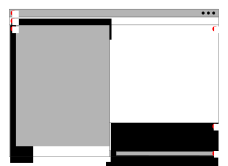
\includegraphics[width=\linewidth]{build/gui/main_view_initial.png}}
\captionof{figure}{Hauptfenster unmittelbar nach dem Starten des Programms}
\end{minipage}

Das Hauptfenster besteht aus der Fensterleiste (A), der Menüleiste (1), dem Editor (2), der Visualisierungsbox (3), der Konsole (4) und dem Eingabefeld (5).
Dabei ist die Fensterleiste kein Bestandteil des eigentlichen Programms; sie ist von der graphischen Oberfläche des Betriebssystems vorgegeben.
Das Eingabefeld ist noch deaktiviert (angedeutet durch die graue Färbung), da noch kein Prolog-Programm geparst wurde.

\subsection{\enquote{Datei}-Menü}

\begin{minipage}{\linewidth}
\makebox[\linewidth]{
    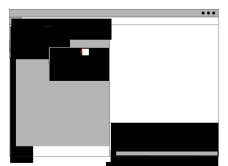
\includegraphics[width=\linewidth]{build/gui/main_view_filemenu.png}}
\captionof{figure}{Hauptfenster mit ausgewähltem \enquote{Datei}-Menü}
\end{minipage}

Das \enquote{Datei}-Menü (1) hat die Einträge \enquote{Öffnen}, \enquote{Speichern}, \enquote{Speichern als...}, \enquote{Zuletzt verwendet} und \enquote{Beenden}.
\enquote{Öffnen} und \enquote{Speichern} führen die jeweiligen Funktionen aus; während \enquote{Speichern} nur bei neu angelegten Prolog-Programmen einen Auswahldialog anzeigt, zeigt \enquote{Speichern als...} immer einen Auswahldialog an.
\enquote{Beenden} beendet das Programm.
\enquote{Zuletzt verwendet} enthält eine Liste von bis zu fünf zuletzt verwendeten Programmen (2).

\subsection{Geöffnete Datei}

\begin{minipage}{\linewidth}
\makebox[\linewidth]{
    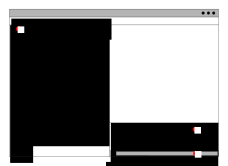
\includegraphics[width=\linewidth]{build/gui/main_view_opened.png}}
\captionof{figure}{Hauptfenster nach dem Öffnen des Beispielprogramms}
\end{minipage}

Nach dem Öffnen des Beispielprogramms wird deren Inhalt im Editor angezeigt (1).
Die Konsole gibt eine entsprechende Meldung aus (2).
Das Eingabefeld bleibt weiterhin deaktiviert (3).

\subsection{Parsen fehlgeschlagen}

\begin{minipage}{\linewidth}
\makebox[\linewidth]{
    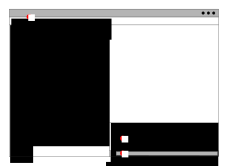
\includegraphics[width=\linewidth]{build/gui/main_view_parse_fail.png}
}
\captionof{figure}{Hauptfenster nach Klick auf \enquote{Parsen}, mit inkorrektem Prolog-Programm}
\end{minipage}

Klickt der Nutzer auf \enquote{Parsen} (1), versucht der Parser das Prolog-Programm im Editor zu verarbeiten.
Stößt er dabei auf Fehler, wird eine Fehlermeldung in der Konsole angezeigt (2).
Das Eingabefeld bleibt weiterhin deaktiviert (3).

\subsection{Parsen erfolgreich}

\begin{minipage}{\linewidth}
\makebox[\linewidth]{

\includegraphics[width=\linewidth]{build/gui/main_view_parse_success.png}
}
\captionof{figure}{Hauptfenster nach Klick auf \enquote{Parsen}, mit korrektem Prolog-Programm}
\end{minipage}

Klickt der Nutzer auf \enquote{Parsen} (1), versucht der Parser das Prolog-Programm im Editor zu verarbeiten.
Treten dabei keine Fehler auf, wird eine entsprechende Meldung in der Konsole angezeigt (2).
Das Eingabefeld wird aktiviert; der Nutzer kann jetzt Abfragen eingeben (3).

\subsection{Fehlerhafte Abfrage}

\begin{minipage}{\linewidth}
\makebox[\linewidth]{

\includegraphics[width=\linewidth]{build/gui/main_view_question_fail.png}
}
\captionof{figure}{Hauptfenster nach fehlerhafter Abfrage im Eingabefeld}
\end{minipage}

Gibt der Nutzer eine Abfrage im Eingabefeld ein (1), versucht der Parser, diese Eingabe zu einem einzelnen Ziel zu verarbeiten.
Stößt er dabei auf Fehler, wird eine Fehlermeldung in der Konsole angezeigt (2).

\subsection{Erfolgreiche Abfrage}

\begin{minipage}{\linewidth}
\makebox[\linewidth]{
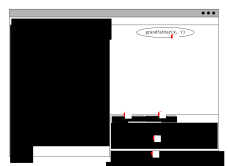
\includegraphics[width=\linewidth]{build/gui/main_view_visualisation_root.png}
}
\captionof{figure}{Hauptfenster nach Eingabe einer Abfrage}
\end{minipage}

Gibt der Nutzer eine Abfrage (1) im Eingabefeld ein, versucht der Parser, diese Eingabe zu einem einzelnen Ziel zu verarbeiten.
Treten dabei keine Fehler auf, wird eine Meldung in der Konsole angezeigt (2) und die Visualisierung der Abarbeitung dieser Abfrage gestartet (3).
Eine Leiste mit Schaltflächen, die zur Steuerung der Visualisierung dienen, wird angezeigt.
Die Schaltfäche \enquote{Nächster Schritt} (4) bewirkt die Ausführung und Visualisierung des nächsten Schrittes.
Die Schaltfläche \enquote{Größer} und \enquote{Kleiner} (5) dienen zum Zoomen in der Visualisierung.

\subsection{Visualisierung}

Um die Beispiele besser darzustellen, wurden sie hier ohne die graphische Oberfläche des Programms eingefügt.
Die visualisierte Abfrage ist \texttt{grandfather(X, Y)} im Beispielprogramm.

\subsubsection{Wurzel}

\begin{minipage}{\linewidth}
\makebox[\linewidth]{
\includegraphics[width=\linewidth]{build/visualisation/01_root.png}
}
\captionof{figure}{Wurzel des Visualisierungsbaumes}
\end{minipage}

Die Wurzel des Visualisierungsbaumes stellt die eingegebene Abfrage dar.

\subsubsection{Fehlgeschlagene Unifikation}

Im nächsten Schritt versucht der Interpreter die Unifikation von \texttt{grandfather(X, Y)} mit dem Fakt \texttt{father(abe, homer)}.
Diese schlägt fehl.

\begin{minipage}{\linewidth}
\makebox[\linewidth]{
\includegraphics[width=\linewidth]{build/visualisation/02_root_fail.png}
}
\captionof{figure}{Eine fehlgeschlagene Unifikation}
\end{minipage}

Die Visualisierung stellt zu unifizierende Ziele als Runde Knoten dar.
Unifikationen werden in  Rechtecken dargestellt, die in zwei weitere rechtecke aufgeteilt sind.
Dabei enthält jede Unifikation im oberen Rechteck den Fakt, mit dem unifiziert werden soll.
Fehlgeschlagene Unifikationen enthalten im unteren Rechteck den Satz "Unifikation fehlgeschlagen:" und den Grund des Fehlschlages.
Außerdem sind sie rot eingefärbt.

\subsubsection{Erfolgreiche Unifikation und Teilziele}

In den weiteren Schritten schlagen die Unifikationen von \texttt{grandfather(X, Y)} mit \texttt{father(homer, bart)}, \texttt{father(homer, lisa)} und \texttt{mother(marge, bart)} fehl.
Die Unifikation mit der Regel \texttt{grandfather(X, Y)} ist erfolgreich.
Dabei werden die Variablennamen durch neue, eindeutige Namen ersetzt um Konflikte zu vermeiden.

\begin{minipage}{\linewidth}
\makebox[\linewidth]{
\includegraphics[width=\linewidth]{build/visualisation/03_root_success.png}
}
\captionof{figure}{Eine erfolgreiche Unifikation mit Einfügung der Teilziele}
\end{minipage}

Erfolgreiche Unifikationen enthalten im unteren Rechteck die resultierenden Substitutionen.
Außerdem sind sie grün eingefärbt.

War eine Unifikation mit einer Regel erfolgreich, so werden ihre Teilziele als neue Ziele, also runde Knoten, zum Graphen hinzugefügt.
Die Substitutionen werden in den Teilzielen angewendet und hervorgehoben.
Die Unifikation und ihre Teilziele werden durch gestrichelte Kanten verbunden.
Dadurch werden im Baum die Fälle \enquote{Ziel wurde unifiziert mit} und \enquote{Ziel ist Teilziel von Regel} unterschieden.

\subsubsection{Erfolgreiche Unifikation mit rückwirkender Substitution}

Im nächsten Schritt steigt der Interpreter in die Teilziele ab und versucht, von links nach rechts diese mit einem Fakt zu unifizieren.

\begin{minipage}{\linewidth}
\makebox[\linewidth]{
\includegraphics[width=\linewidth]{build/visualisation/04_subgoal_father_success.png}
}
\captionof{figure}{Eine erfolgreiche Unifikation mit mit rückwirkender Substitution}
\end{minipage}

In diesem Beispiel ist der gefundene Fakt keine Regel, hat also keine Teilziele.
Trotzdem müssen die Substitutionen in der restlichen Teilzielen angewendet werden.
Die angewendeten Substitutionen werden dabei in den betreffenden Zielen hervorgehoben.

\subsubsection{Backtracking}

Hier wurden einige Schritte übersprungen.
Das zweite Teilziel wurde mit der ersten Definition von \texttt{parent(X, Y)} unifiziert.
Diese hat als Teilziel \texttt{mother(X, Y)}.
Mit der Belegung \texttt{X = homer} gibt es dafür aber keine Lösung.
Der Interpreter muss also nach einer alternativen Definition von \texttt{parent} suchen und dazu zurückspringen (\enquote{Backtracking}).

\begin{minipage}{\linewidth}
\makebox[\linewidth]{
\includegraphics[width=\linewidth]{build/visualisation/09_mother_backtrack.png}
}
\captionof{figure}{Rücksprung nachdem ein Ziel nicht erfüllbar ist}
\end{minipage}

Ein Rücksprung wird durch eine aus Punkten bestehende, rot eingefärbte Karte dargestellt.
Das nicht erfüllbare Teilziel wird ebenfalls rot eingefärbt und mit dem Text \enquote{Nicht erfüllbar!} ergänzt.

\section{Glossar}

\textbf{Nutzer}:
Eine Person, welche den Dienst nutzt.

\end{document}
